\documentclass[11pt,a4paper,oneside]{report}   
\usepackage{listings}
\linespread{1.5}
%%%%%%%%%%%%%%%%%%%%%%%%%%%%%%%%%
% PACKAGE IMPORTS
%%%%%%%%%%%%%%%%%%%%%%%%%%%%%%%%%


\usepackage[tmargin=2cm,rmargin=1in,lmargin=1in,margin=0.85in,bmargin=2cm,footskip=.2in]{geometry}
\usepackage{amsmath,amsfonts,amsthm,amssymb,mathtools}
\usepackage[varbb]{newpxmath}
\usepackage{xfrac}
\usepackage[makeroom]{cancel}
\usepackage{mathtools}
\usepackage{bookmark}
\usepackage{enumitem}
\usepackage{hyperref,theoremref}
\hypersetup{
	pdftitle={Assignment},
	colorlinks=true, linkcolor=doc!90,
	bookmarksnumbered=true,
	bookmarksopen=true
}
\usepackage[most,many,breakable]{tcolorbox}
\usepackage{xcolor}
\usepackage{varwidth}
\usepackage{varwidth}
\usepackage{etoolbox}
%\usepackage{authblk}
\usepackage{nameref}
\usepackage{multicol,array}
\usepackage{tikz-cd}
\usepackage[ruled,vlined,linesnumbered]{algorithm2e}
\usepackage{comment} % enables the use of multi-line comments (\ifx \fi) 
\usepackage{import}
\usepackage{xifthen}
\usepackage{pdfpages}
\usepackage{transparent}

\newcommand\mycommfont[1]{\footnotesize\ttfamily\textcolor{blue}{#1}}
\SetCommentSty{mycommfont}
\newcommand{\incfig}[1]{%
	\def\svgwidth{\columnwidth}
	\import{./figures/}{#1.pdf_tex}
}

\usepackage{tikzsymbols}
\renewcommand\qedsymbol{$\Laughey$}


%\usepackage{import}
%\usepackage{xifthen}
%\usepackage{pdfpages}
%\usepackage{transparent}


%%%%%%%%%%%%%%%%%%%%%%%%%%%%%%
% SELF MADE COLORS
%%%%%%%%%%%%%%%%%%%%%%%%%%%%%%



\definecolor{myg}{RGB}{56, 140, 70}
\definecolor{myb}{RGB}{45, 111, 177}
\definecolor{myr}{RGB}{199, 68, 64}
\definecolor{mytheorembg}{HTML}{F2F2F9}
\definecolor{mytheoremfr}{HTML}{00007B}
\definecolor{mylenmabg}{HTML}{FFFAF8}
\definecolor{mylenmafr}{HTML}{983b0f}
\definecolor{mypropbg}{HTML}{f2fbfc}
\definecolor{mypropfr}{HTML}{191971}
\definecolor{myexamplebg}{HTML}{F2FBF8}
\definecolor{myexamplefr}{HTML}{88D6D1}
\definecolor{myexampleti}{HTML}{2A7F7F}
\definecolor{mydefinitbg}{HTML}{E5E5FF}
\definecolor{mydefinitfr}{HTML}{3F3FA3}
\definecolor{notesgreen}{RGB}{0,162,0}
\definecolor{myp}{RGB}{197, 92, 212}
\definecolor{mygr}{HTML}{2C3338}
\definecolor{myred}{RGB}{127,0,0}
\definecolor{myyellow}{RGB}{169,121,69}
\definecolor{myexercisebg}{HTML}{F2FBF8}
\definecolor{myexercisefg}{HTML}{88D6D1}


%%%%%%%%%%%%%%%%%%%%%%%%%%%%
% TCOLORBOX SETUPS
%%%%%%%%%%%%%%%%%%%%%%%%%%%%

\setlength{\parindent}{1cm}
%================================
% THEOREM BOX
%================================

\tcbuselibrary{theorems,skins,hooks}
\newtcbtheorem[number within=section]{Theorem}{Theorem}
{%
	enhanced,
	breakable,
	colback = mytheorembg,
	frame hidden,
	boxrule = 0sp,
	borderline west = {2pt}{0pt}{mytheoremfr},
	sharp corners,
	detach title,
	before upper = \tcbtitle\par\smallskip,
	coltitle = mytheoremfr,
	fonttitle = \bfseries\sffamily,
	description font = \mdseries,
	separator sign none,
	segmentation style={solid, mytheoremfr},
}
{th}

\tcbuselibrary{theorems,skins,hooks}
\newtcbtheorem[number within=chapter]{theorem}{Theorem}
{%
	enhanced,
	breakable,
	colback = mytheorembg,
	frame hidden,
	boxrule = 0sp,
	borderline west = {2pt}{0pt}{mytheoremfr},
	sharp corners,
	detach title,
	before upper = \tcbtitle\par\smallskip,
	coltitle = mytheoremfr,
	fonttitle = \bfseries\sffamily,
	description font = \mdseries,
	separator sign none,
	segmentation style={solid, mytheoremfr},
}
{th}


\tcbuselibrary{theorems,skins,hooks}
\newtcolorbox{Theoremcon}
{%
	enhanced
	,breakable
	,colback = mytheorembg
	,frame hidden
	,boxrule = 0sp
	,borderline west = {2pt}{0pt}{mytheoremfr}
	,sharp corners
	,description font = \mdseries
	,separator sign none
}

%================================
% Corollery
%================================
\tcbuselibrary{theorems,skins,hooks}
\newtcbtheorem[number within=section]{Corollary}{Corollary}
{%
	enhanced
	,breakable
	,colback = myp!10
	,frame hidden
	,boxrule = 0sp
	,borderline west = {2pt}{0pt}{myp!85!black}
	,sharp corners
	,detach title
	,before upper = \tcbtitle\par\smallskip
	,coltitle = myp!85!black
	,fonttitle = \bfseries\sffamily
	,description font = \mdseries
	,separator sign none
	,segmentation style={solid, myp!85!black}
}
{th}
\tcbuselibrary{theorems,skins,hooks}
\newtcbtheorem[number within=chapter]{corollary}{Corollary}
{%
	enhanced
	,breakable
	,colback = myp!10
	,frame hidden
	,boxrule = 0sp
	,borderline west = {2pt}{0pt}{myp!85!black}
	,sharp corners
	,detach title
	,before upper = \tcbtitle\par\smallskip
	,coltitle = myp!85!black
	,fonttitle = \bfseries\sffamily
	,description font = \mdseries
	,separator sign none
	,segmentation style={solid, myp!85!black}
}
{th}


%================================
% LENMA
%================================

\tcbuselibrary{theorems,skins,hooks}
\newtcbtheorem[number within=section]{Lenma}{Lenma}
{%
	enhanced,
	breakable,
	colback = mylenmabg,
	frame hidden,
	boxrule = 0sp,
	borderline west = {2pt}{0pt}{mylenmafr},
	sharp corners,
	detach title,
	before upper = \tcbtitle\par\smallskip,
	coltitle = mylenmafr,
	fonttitle = \bfseries\sffamily,
	description font = \mdseries,
	separator sign none,
	segmentation style={solid, mylenmafr},
}
{th}

\tcbuselibrary{theorems,skins,hooks}
\newtcbtheorem[number within=chapter]{lenma}{Lenma}
{%
	enhanced,
	breakable,
	colback = mylenmabg,
	frame hidden,
	boxrule = 0sp,
	borderline west = {2pt}{0pt}{mylenmafr},
	sharp corners,
	detach title,
	before upper = \tcbtitle\par\smallskip,
	coltitle = mylenmafr,
	fonttitle = \bfseries\sffamily,
	description font = \mdseries,
	separator sign none,
	segmentation style={solid, mylenmafr},
}
{th}


%================================
% PROPOSITION
%================================

\tcbuselibrary{theorems,skins,hooks}
\newtcbtheorem[number within=section]{Prop}{Proposition}
{%
	enhanced,
	breakable,
	colback = mypropbg,
	frame hidden,
	boxrule = 0sp,
	borderline west = {2pt}{0pt}{mypropfr},
	sharp corners,
	detach title,
	before upper = \tcbtitle\par\smallskip,
	coltitle = mypropfr,
	fonttitle = \bfseries\sffamily,
	description font = \mdseries,
	separator sign none,
	segmentation style={solid, mypropfr},
}
{th}

\tcbuselibrary{theorems,skins,hooks}
\newtcbtheorem[number within=chapter]{prop}{Proposition}
{%
	enhanced,
	breakable,
	colback = mypropbg,
	frame hidden,
	boxrule = 0sp,
	borderline west = {2pt}{0pt}{mypropfr},
	sharp corners,
	detach title,
	before upper = \tcbtitle\par\smallskip,
	coltitle = mypropfr,
	fonttitle = \bfseries\sffamily,
	description font = \mdseries,
	separator sign none,
	segmentation style={solid, mypropfr},
}
{th}


%================================
% CLAIM
%================================

\tcbuselibrary{theorems,skins,hooks}
\newtcbtheorem[number within=section]{claim}{Claim}
{%
	enhanced
	,breakable
	,colback = myg!10
	,frame hidden
	,boxrule = 0sp
	,borderline west = {2pt}{0pt}{myg}
	,sharp corners
	,detach title
	,before upper = \tcbtitle\par\smallskip
	,coltitle = myg!85!black
	,fonttitle = \bfseries\sffamily
	,description font = \mdseries
	,separator sign none
	,segmentation style={solid, myg!85!black}
}
{th}



%================================
% Exercise
%================================

\tcbuselibrary{theorems,skins,hooks}
\newtcbtheorem[number within=section]{Exercise}{Exercise}
{%
	enhanced,
	breakable,
	colback = myexercisebg,
	frame hidden,
	boxrule = 0sp,
	borderline west = {2pt}{0pt}{myexercisefg},
	sharp corners,
	detach title,
	before upper = \tcbtitle\par\smallskip,
	coltitle = myexercisefg,
	fonttitle = \bfseries\sffamily,
	description font = \mdseries,
	separator sign none,
	segmentation style={solid, myexercisefg},
}
{th}

\tcbuselibrary{theorems,skins,hooks}
\newtcbtheorem[number within=chapter]{exercise}{Exercise}
{%
	enhanced,
	breakable,
	colback = myexercisebg,
	frame hidden,
	boxrule = 0sp,
	borderline west = {2pt}{0pt}{myexercisefg},
	sharp corners,
	detach title,
	before upper = \tcbtitle\par\smallskip,
	coltitle = myexercisefg,
	fonttitle = \bfseries\sffamily,
	description font = \mdseries,
	separator sign none,
	segmentation style={solid, myexercisefg},
}
{th}

%================================
% EXAMPLE BOX
%================================

\newtcbtheorem[number within=section]{Example}{Example}
{%
	colback = myexamplebg
	,breakable
	,colframe = myexamplefr
	,coltitle = myexampleti
	,boxrule = 1pt
	,sharp corners
	,detach title
	,before upper=\tcbtitle\par\smallskip
	,fonttitle = \bfseries
	,description font = \mdseries
	,separator sign none
	,description delimiters parenthesis
}
{ex}

\newtcbtheorem[number within=chapter]{example}{Example}
{%
	colback = myexamplebg
	,breakable
	,colframe = myexamplefr
	,coltitle = myexampleti
	,boxrule = 1pt
	,sharp corners
	,detach title
	,before upper=\tcbtitle\par\smallskip
	,fonttitle = \bfseries
	,description font = \mdseries
	,separator sign none
	,description delimiters parenthesis
}
{ex}

%================================
% DEFINITION BOX
%================================

\newtcbtheorem[number within=section]{Definition}{Definition}{enhanced,
	before skip=2mm,after skip=2mm, colback=red!5,colframe=red!80!black,boxrule=0.5mm,
	attach boxed title to top left={xshift=1cm,yshift*=1mm-\tcboxedtitleheight}, varwidth boxed title*=-3cm,
	boxed title style={frame code={
					\path[fill=tcbcolback]
					([yshift=-1mm,xshift=-1mm]frame.north west)
					arc[start angle=0,end angle=180,radius=1mm]
					([yshift=-1mm,xshift=1mm]frame.north east)
					arc[start angle=180,end angle=0,radius=1mm];
					\path[left color=tcbcolback!60!black,right color=tcbcolback!60!black,
						middle color=tcbcolback!80!black]
					([xshift=-2mm]frame.north west) -- ([xshift=2mm]frame.north east)
					[rounded corners=1mm]-- ([xshift=1mm,yshift=-1mm]frame.north east)
					-- (frame.south east) -- (frame.south west)
					-- ([xshift=-1mm,yshift=-1mm]frame.north west)
					[sharp corners]-- cycle;
				},interior engine=empty,
		},
	fonttitle=\bfseries,
	title={#2},#1}{def}
\newtcbtheorem[number within=chapter]{definition}{Definition}{enhanced,
	before skip=2mm,after skip=2mm, colback=red!5,colframe=red!80!black,boxrule=0.5mm,
	attach boxed title to top left={xshift=1cm,yshift*=1mm-\tcboxedtitleheight}, varwidth boxed title*=-3cm,
	boxed title style={frame code={
					\path[fill=tcbcolback]
					([yshift=-1mm,xshift=-1mm]frame.north west)
					arc[start angle=0,end angle=180,radius=1mm]
					([yshift=-1mm,xshift=1mm]frame.north east)
					arc[start angle=180,end angle=0,radius=1mm];
					\path[left color=tcbcolback!60!black,right color=tcbcolback!60!black,
						middle color=tcbcolback!80!black]
					([xshift=-2mm]frame.north west) -- ([xshift=2mm]frame.north east)
					[rounded corners=1mm]-- ([xshift=1mm,yshift=-1mm]frame.north east)
					-- (frame.south east) -- (frame.south west)
					-- ([xshift=-1mm,yshift=-1mm]frame.north west)
					[sharp corners]-- cycle;
				},interior engine=empty,
		},
	fonttitle=\bfseries,
	title={#2},#1}{def}



%================================
% Solution BOX
%================================

\makeatletter
\newtcbtheorem{question}{Question}{enhanced,
	breakable,
	colback=white,
	colframe=myb!80!black,
	attach boxed title to top left={yshift*=-\tcboxedtitleheight},
	fonttitle=\bfseries,
	title={#2},
	boxed title size=title,
	boxed title style={%
			sharp corners,
			rounded corners=northwest,
			colback=tcbcolframe,
			boxrule=0pt,
		},
	underlay boxed title={%
			\path[fill=tcbcolframe] (title.south west)--(title.south east)
			to[out=0, in=180] ([xshift=5mm]title.east)--
			(title.center-|frame.east)
			[rounded corners=\kvtcb@arc] |-
			(frame.north) -| cycle;
		},
	#1
}{def}
\makeatother

%================================
% SOLUTION BOX
%================================

\makeatletter
\newtcolorbox{solution}{enhanced,
	breakable,
	colback=white,
	colframe=myg!80!black,
	attach boxed title to top left={yshift*=-\tcboxedtitleheight},
	title=Solution,
	boxed title size=title,
	boxed title style={%
			sharp corners,
			rounded corners=northwest,
			colback=tcbcolframe,
			boxrule=0pt,
		},
	underlay boxed title={%
			\path[fill=tcbcolframe] (title.south west)--(title.south east)
			to[out=0, in=180] ([xshift=5mm]title.east)--
			(title.center-|frame.east)
			[rounded corners=\kvtcb@arc] |-
			(frame.north) -| cycle;
		},
}
\makeatother

%================================
% Question BOX
%================================

\makeatletter
\newtcbtheorem{qstion}{Question}{enhanced,
	breakable,
	colback=white,
	colframe=mygr,
	attach boxed title to top left={yshift*=-\tcboxedtitleheight},
	fonttitle=\bfseries,
	title={#2},
	boxed title size=title,
	boxed title style={%
			sharp corners,
			rounded corners=northwest,
			colback=tcbcolframe,
			boxrule=0pt,
		},
	underlay boxed title={%
			\path[fill=tcbcolframe] (title.south west)--(title.south east)
			to[out=0, in=180] ([xshift=5mm]title.east)--
			(title.center-|frame.east)
			[rounded corners=\kvtcb@arc] |-
			(frame.north) -| cycle;
		},
	#1
}{def}
\makeatother

\newtcbtheorem[number within=chapter]{wconc}{Wrong Concept}{
	breakable,
	enhanced,
	colback=white,
	colframe=myr,
	arc=0pt,
	outer arc=0pt,
	fonttitle=\bfseries\sffamily\large,
	colbacktitle=myr,
	attach boxed title to top left={},
	boxed title style={
			enhanced,
			skin=enhancedfirst jigsaw,
			arc=3pt,
			bottom=0pt,
			interior style={fill=myr}
		},
	#1
}{def}



%================================
% NOTE BOX
%================================

\usetikzlibrary{arrows,calc,shadows.blur}
\tcbuselibrary{skins}
\newtcolorbox{note}[1][]{%
	enhanced jigsaw,
	colback=gray!20!white,%
	colframe=gray!80!black,
	size=small,
	boxrule=1pt,
	title=\textbf{Note:-},
	halign title=flush center,
	coltitle=black,
	breakable,
	drop shadow=black!50!white,
	attach boxed title to top left={xshift=1cm,yshift=-\tcboxedtitleheight/2,yshifttext=-\tcboxedtitleheight/2},
	minipage boxed title=1.5cm,
	boxed title style={%
			colback=white,
			size=fbox,
			boxrule=1pt,
			boxsep=2pt,
			underlay={%
					\coordinate (dotA) at ($(interior.west) + (-0.5pt,0)$);
					\coordinate (dotB) at ($(interior.east) + (0.5pt,0)$);
					\begin{scope}
						\clip (interior.north west) rectangle ([xshift=3ex]interior.east);
						\filldraw [white, blur shadow={shadow opacity=60, shadow yshift=-.75ex}, rounded corners=2pt] (interior.north west) rectangle (interior.south east);
					\end{scope}
					\begin{scope}[gray!80!black]
						\fill (dotA) circle (2pt);
						\fill (dotB) circle (2pt);
					\end{scope}
				},
		},
	#1,
}

%%%%%%%%%%%%%%%%%%%%%%%%%%%%%%
% SELF MADE COMMANDS
%%%%%%%%%%%%%%%%%%%%%%%%%%%%%%


\newcommand{\thm}[2]{\begin{Theorem}{#1}{}#2\end{Theorem}}
\newcommand{\cor}[2]{\begin{Corollary}{#1}{}#2\end{Corollary}}
\newcommand{\mlenma}[2]{\begin{Lenma}{#1}{}#2\end{Lenma}}
\newcommand{\mprop}[2]{\begin{Prop}{#1}{}#2\end{Prop}}
\newcommand{\clm}[3]{\begin{claim}{#1}{#2}#3\end{claim}}
\newcommand{\wc}[2]{\begin{wconc}{#1}{}\setlength{\parindent}{1cm}#2\end{wconc}}
\newcommand{\thmcon}[1]{\begin{Theoremcon}{#1}\end{Theoremcon}}
\newcommand{\ex}[2]{\begin{Example}{#1}{}#2\end{Example}}
\newcommand{\dfn}[2]{\begin{Definition}[colbacktitle=red!75!black]{#1}{}#2\end{Definition}}
\newcommand{\dfnc}[2]{\begin{definition}[colbacktitle=red!75!black]{#1}{}#2\end{definition}}
\newcommand{\qs}[2]{\begin{question}{#1}{}#2\end{question}}
\newcommand{\pf}[2]{\begin{myproof}[#1]#2\end{myproof}}
\newcommand{\nt}[1]{\begin{note}#1\end{note}}

\newcommand*\circled[1]{\tikz[baseline=(char.base)]{
		\node[shape=circle,draw,inner sep=1pt] (char) {#1};}}
\newcommand\getcurrentref[1]{%
	\ifnumequal{\value{#1}}{0}
	{??}
	{\the\value{#1}}%
}
\newcommand{\getCurrentSectionNumber}{\getcurrentref{section}}
\newenvironment{myproof}[1][\proofname]{%
	\proof[\bfseries #1: ]%
}{\endproof}

\newcommand{\mclm}[2]{\begin{myclaim}[#1]#2\end{myclaim}}
\newenvironment{myclaim}[1][\claimname]{\proof[\bfseries #1: ]}{}

\newcounter{mylabelcounter}

\makeatletter
\newcommand{\setword}[2]{%
	\phantomsection
	#1\def\@currentlabel{\unexpanded{#1}}\label{#2}%
}
\makeatother




\tikzset{
	symbol/.style={
			draw=none,
			every to/.append style={
					edge node={node [sloped, allow upside down, auto=false]{$#1$}}}
		}
}


% deliminators
\DeclarePairedDelimiter{\abs}{\lvert}{\rvert}
\DeclarePairedDelimiter{\norm}{\lVert}{\rVert}

\DeclarePairedDelimiter{\ceil}{\lceil}{\rceil}
\DeclarePairedDelimiter{\floor}{\lfloor}{\rfloor}
\DeclarePairedDelimiter{\round}{\lfloor}{\rceil}

\newsavebox\diffdbox
\newcommand{\slantedromand}{{\mathpalette\makesl{d}}}
\newcommand{\makesl}[2]{%
	\begingroup
	\sbox{\diffdbox}{$\mathsurround=0pt#1\mathrm{#2}$}%
	\pdfsave
	\pdfsetmatrix{1 0 0.2 1}%
	\rlap{\usebox{\diffdbox}}%
	\pdfrestore
	\hskip\wd\diffdbox
	\endgroup
}
\newcommand{\dd}[1][]{\ensuremath{\mathop{}\!\ifstrempty{#1}{%
			\slantedromand\@ifnextchar^{\hspace{0.2ex}}{\hspace{0.1ex}}}%
		{\slantedromand\hspace{0.2ex}^{#1}}}}
\ProvideDocumentCommand\dv{o m g}{%
	\ensuremath{%
		\IfValueTF{#3}{%
			\IfNoValueTF{#1}{%
				\frac{\dd #2}{\dd #3}%
			}{%
				\frac{\dd^{#1} #2}{\dd #3^{#1}}%
			}%
		}{%
			\IfNoValueTF{#1}{%
				\frac{\dd}{\dd #2}%
			}{%
				\frac{\dd^{#1}}{\dd #2^{#1}}%
			}%
		}%
	}%
}
\providecommand*{\pdv}[3][]{\frac{\partial^{#1}#2}{\partial#3^{#1}}}
%  - others
\DeclareMathOperator{\Lap}{\mathcal{L}}
\DeclareMathOperator{\Var}{Var} % varience
\DeclareMathOperator{\Cov}{Cov} % covarience
\DeclareMathOperator{\E}{E} % expected

% Since the amsthm package isn't loaded

% I prefer the slanted \leq
\let\oldleq\leq % save them in case they're every wanted
\let\oldgeq\geq
\renewcommand{\leq}{\leqslant}
\renewcommand{\geq}{\geqslant}

% % redefine matrix env to allow for alignment, use r as default
% \renewcommand*\env@matrix[1][r]{\hskip -\arraycolsep
%     \let\@ifnextchar\new@ifnextchar
%     \array{*\c@MaxMatrixCols #1}}


%\usepackage{framed}
%\usepackage{titletoc}
%\usepackage{etoolbox}
%\usepackage{lmodern}


%\patchcmd{\tableofcontents}{\contentsname}{\sffamily\contentsname}{}{}

%\renewenvironment{leftbar}
%{\def\FrameCommand{\hspace{6em}%
%		{\color{myyellow}\vrule width 2pt depth 6pt}\hspace{1em}}%
%	\MakeFramed{\parshape 1 0cm \dimexpr\textwidth-6em\relax\FrameRestore}\vskip2pt%
%}
%{\endMakeFramed}

%\titlecontents{chapter}
%[0em]{\vspace*{2\baselineskip}}
%{\parbox{4.5em}{%
%		\hfill\Huge\sffamily\bfseries\color{myred}\thecontentspage}%
%	\vspace*{-2.3\baselineskip}\leftbar\textsc{\small\chaptername~\thecontentslabel}\\\sffamily}
%{}{\endleftbar}
%\titlecontents{section}
%[8.4em]
%{\sffamily\contentslabel{3em}}{}{}
%{\hspace{0.5em}\nobreak\itshape\color{myred}\contentspage}
%\titlecontents{subsection}
%[8.4em]
%{\sffamily\contentslabel{3em}}{}{}  
%{\hspace{0.5em}\nobreak\itshape\color{myred}\contentspage}



%%%%%%%%%%%%%%%%%%%%%%%%%%%%%%%%%%%%%%%%%%%
% TABLE OF CONTENTS
%%%%%%%%%%%%%%%%%%%%%%%%%%%%%%%%%%%%%%%%%%%

\usepackage{tikz}
\definecolor{doc}{RGB}{0,60,110}
\usepackage{titletoc}
\contentsmargin{0cm}
\titlecontents{chapter}[3.7pc]
{\addvspace{30pt}%
	\begin{tikzpicture}[remember picture, overlay]%
		\draw[fill=doc!60,draw=doc!60] (-7,-.1) rectangle (-0.9,.5);%
		\pgftext[left,x=-3.5cm,y=0.2cm]{\color{white}\Large\sc\bfseries Chapter\ \thecontentslabel};%
	\end{tikzpicture}\color{doc!60}\large\sc\bfseries}%
{}
{}
{\;\titlerule\;\large\sc\bfseries Page \thecontentspage
	\begin{tikzpicture}[remember picture, overlay]
		\draw[fill=doc!60,draw=doc!60] (2pt,0) rectangle (4,0.1pt);
	\end{tikzpicture}}%
\titlecontents{section}[3.7pc]
{\addvspace{2pt}}
{\contentslabel[\thecontentslabel]{2pc}}
{}
{\hfill\small \thecontentspage}
[]
\titlecontents*{subsection}[3.7pc]
{\addvspace{-1pt}\small}
{}
{}
{\ --- \small\thecontentspage}
[ \textbullet\ ][]

\makeatletter
\renewcommand{\tableofcontents}{%
	\chapter*{%
	  \vspace*{-20\p@}%
	  \begin{tikzpicture}[remember picture, overlay]%
		  \pgftext[right,x=15cm,y=0.2cm]{\color{doc!60}\Huge\sc\bfseries \contentsname};%
		  \draw[fill=doc!60,draw=doc!60] (13,-.75) rectangle (20,1);%
		  \clip (13,-.75) rectangle (20,1);
		  \pgftext[right,x=15cm,y=0.2cm]{\color{white}\Huge\sc\bfseries \contentsname};%
	  \end{tikzpicture}}%
	\@starttoc{toc}}
\makeatother


\usepackage{graphicx}
\graphicspath{ {./images/} }

\begin{document}
%%TODO: tanszék, konzulens, képzés szép kiíráasa
%%\title{\Huge{MSc - Önálló laboratórium 2}\\Beszámoló\\Amazon Web Services}
%%\author{\huge{Daniel Mark Kiss}}
%%\author{\huge{Gazdaságinformatika}}
%%\author{\huge{Távközlési és Médiainformatikai Tanszék}}
%%\author{\huge{Konzulens: István Pelle}}
%%\date{2023}
\pagenumbering{arabic}
\begin{titlepage}
    \begin{center}
        
\includegraphics[width=60mm,keepaspectratio]{images/BMElogo.png}\\
        \vspace{0.3cm}
        \textbf{Budapest University of Technology and Economics}\\
        \textmd{Faculty of Electrical Engineering and Informatics}\\
        \textmd{Department of Telecommunications and Media Informatics}\\[5cm]

        \vspace{0.4cm}
        {\huge \bfseries Amazon Web Services}\\[0.8cm]
        \vspace{0.5cm}
        \textsc{\Large MSc - Project laboratory 2}\\[0.8cm]
        \vspace{0.5cm}
        \textsc{\Large Report}\\[4cm]

        \begin{tabular}{cc}
            \makebox[7cm]{\emph{Created by}} & \makebox[7cm]{\emph{Supervisor}} \\
            \makebox[7cm]{Dániel Márk Kiss}  & \makebox[7cm]{István Pelle}
        \end{tabular}

        \vfill
        {\large \today}
    \end{center}
\end{titlepage}

%%\maketitle
\newpage
\tableofcontents
\pagebreak

\chapter{Introduction}

Amazon Web Services (AWS) is a comprehensive cloud computing platform provided by Amazon. It includes a mixture of infrastructure-as-a-service (IaaS), platform-as-a-service (PaaS) and packaged-software-as-a-service (SaaS). It offers a vast array of cloud services, including computing power, storage, databases, machine learning, analytics, and more. AWS allows individuals and organizations to access and utilize computing resources over the internet, without the need to own or maintain physical servers and infrastructure.
Amazon launched its first web services in 2002 from the internal infrastructure that Amazon.com built to handle its online retail operations. In 2006, it began offering its defining IaaS services. AWS was one of the first companies to introduce a pay-as-you-go cloud computing model that scales to provide users with compute, storage or throughput as needed.
AWS is separated into different services; each can be configured in different ways based on the user's needs. Users can see configuration options and individual server maps for an AWS service. AWS provides a scalable and flexible environment for businesses to build, deploy, and manage applications and services. It offers a pay-as-you-go pricing model, which means users only pay for the resources they consume, making it cost-effective and efficient for a wide range of use cases. \cite{techtagaws}

\chapter{Current AWS features and techologies}

Before I started the development of the application I have done a course provided by Amazon. It conatains a 14 module class where they teache the fundamentals of AWS.
It was roughly 5 weeks for me to finish and complete all laboratory exercises and module closing quiz. Throughout the course I have familiarised myself with the different AWS services and theoretical background. It proved to be a good repetition for my previous knowledge like REST API. \cite{awsacademy}


\section{Amazon Elastic Compute Cloud (EC2)}

This service provides resizable compute capacity in the cloud, allowing users to run virtual servers, known as "instances," for various computing tasks.
Key features:
\begin{enumerate}
  \item Scalability: EC2 instances can be quickly scaled up or down based on demand. This means that users can add or remove instances to match the needs of their applications or workloads.
  \item Variety of Instance Types: EC2 offers a wide range of instance types optimized for different use cases. These include instances optimized for compute-intensive workloads, memory-intensive tasks, storage-optimized applications, and more.
  \item Operating System Flexibility: Users can choose from a variety of operating systems, including various Linux distributions, Microsoft Windows, and others, to run on their EC2 instances. \cite{awsec2}
\end{enumerate}
\section{Amazon Simple Storage Service (S3)}

S3 offers scalable object storage for storing and retrieving data. It is commonly used for data backup, hosting static websites, and as a storage backend for applications.
Amazon S3 is designed to provide durability, availability, and scalability at a low cost.
Key features:
\begin{enumerate}
  \item Object Storage: Amazon S3 stores data as objects, which consist of a file and its associated metadata. Each object is identified by a unique key, making it easy to access and manage.
  \item Buckets: A bucket is a container for objects stored in Amazon S3. Buckets act as top-level folders or directories for organizing and managing objects. Each bucket has a unique name and is associated with a specific AWS region.
  \item Durability and Availability: Amazon S3 is designed to provide 99.999999999% (11 9's) durability for objects over a given year. It achieves this by replicating data across multiple Availability Zones within a region, ensuring high availability.
  \item Scalability: Amazon S3 can scale to accommodate virtually unlimited amounts of data. Users can easily upload, store, and retrieve any amount of data, making it suitable for a wide range of use cases.
  \item ccess Control: Users can control access to their buckets and objects through AWS Identity and Access Management (IAM) policies, bucket policies, Access Control Lists (ACLs), and signed URLs or cookies.
  \item Cross-Region Replication: Users can configure Amazon S3 to automatically replicate objects from one bucket to another in a different AWS region. This helps achieve geographic redundancy and compliance with data residency requirements.
  \item Static Website Hosting: Amazon S3 can be used to host static websites, providing a cost-effective solution for hosting web content. \cite{awss3}
\end{enumerate}


\section{Amazon RDS (Relational Database Service)}

RDS offers managed database services for various database engines, including MySQL, PostgreSQL, Oracle, and Microsoft SQL Server.
Key features:
\begin{enumerate}
  \item Managed Service: AWS handles the heavy lifting of database administration tasks such as hardware provisioning, database setup, configuration, patch management, and backups. This allows users to focus on application development rather than database management. \cite{awsrds}
\end{enumerate}


\section{Amazon DynamoDB}

A fully-managed NoSQL database service that provides high performance and seamless scalability for applications that require low-latency access to data.
\begin{enumerate}
  \item NoSQL Database: DynamoDB is a NoSQL database, which means it does not rely on a fixed schema like traditional relational databases. This allows for flexible data modeling, making it well-suited for applications with evolving data structures.
  \item Managed Service: AWS handles all the operational aspects of DynamoDB, including hardware provisioning, setup, configuration, and maintenance. This frees developers from the burden of database management tasks.
  \item Scalability: DynamoDB is designed to scale easily, both in terms of read and write throughput. It can handle massive volumes of traffic and automatically scales based on demand. Users can adjust read and write capacity units to accommodate their application's needs. \cite{awsddb}
\end{enumerate}

\section{AWS Lambda}

This service allows users to run code without provisioning or managing servers. It executes code in response to specific events, making it a key component of serverless architecture.
\begin{enumerate}
  \item Serverless Architecture: Lambda is a serverless computing service, which means developers do not need to manage the underlying servers. Instead, they write code and AWS handles the execution and scaling of that code.
  \item Event-Driven Model: Lambda functions are triggered by events such as changes to data in an Amazon S3 bucket, updates to a DynamoDB table, or incoming HTTP requests via Amazon API Gateway. This event-driven model allows for real-time responses to changes in the environment.
  \item Supported Runtimes: AWS Lambda supports multiple programming languages including Node.js, Python, Java, Go, Ruby, .NET Core, and custom runtimes.
        This flexibility enables developers to use their preferred programming language.
  \item Pay-per-Use Pricing: With AWS Lambda, users pay only for the compute time consumed by their code. There is no charge when code is not running. This pricing model can lead to cost savings compared to traditional server-based architectures. \cite{awslambda}
\end{enumerate}


\section{AWS CodeCommit}
AWS CodeCommit is a fully managed source control service provided by Amazon Web Services (AWS). It is a secure and scalable Git-based repository hosting service designed to help teams collaborate on code development and version control. CodeCommit provides a secure and reliable platform for storing and managing code repositories.

Key features:
\begin{enumerate}
  \item Git Repository Hosting: CodeCommit supports the Git version control system, providing a familiar interface for developers to manage their code repositories.
  \item Secure and Private: CodeCommit repositories are secure by default and can be configured to be private. Access control policies, AWS Identity and Access Management (IAM) permissions, and encryption options ensure the confidentiality and integrity of code.
  \item Integration with AWS Services: CodeCommit seamlessly integrates with other AWS services, such as AWS CodePipeline, AWS CodeBuild, AWS CodeDeploy, AWS CloudFormation, and more. This enables end-to-end continuous integration and continuous deployment (CI/CD) workflows.
  \item Version Control: CodeCommit allows multiple developers to collaborate on projects by providing version control capabilities. Developers can create branches, merge code changes, and track commit history. \cite{awscodecommit}
\end{enumerate}



\chapter{Development}

\section{Overview}
For the development phase of the project I used AWS's Cloud9 integrated developer environment(IDE) as the main developer platform for the front-end.
I have also version controled the whole development process using git and publishing it on GitHub and also Amazons Code Commit system. Not only the source code can be found there but also the documentation of this project as I have writen it using \LaTeX{}.
The project I have created using AWS and other technologies is a Book Tracking website. It has a seperate admin page where the admins can register the users and another page where the users can track their books.
For the books there are three state. Not started, Reading and Finished. These books are presented in a crad format and it is only visible to the users after a successful login.
To achive this I have used the following technologies:

\begin{figure}[!ht]
  \centering
  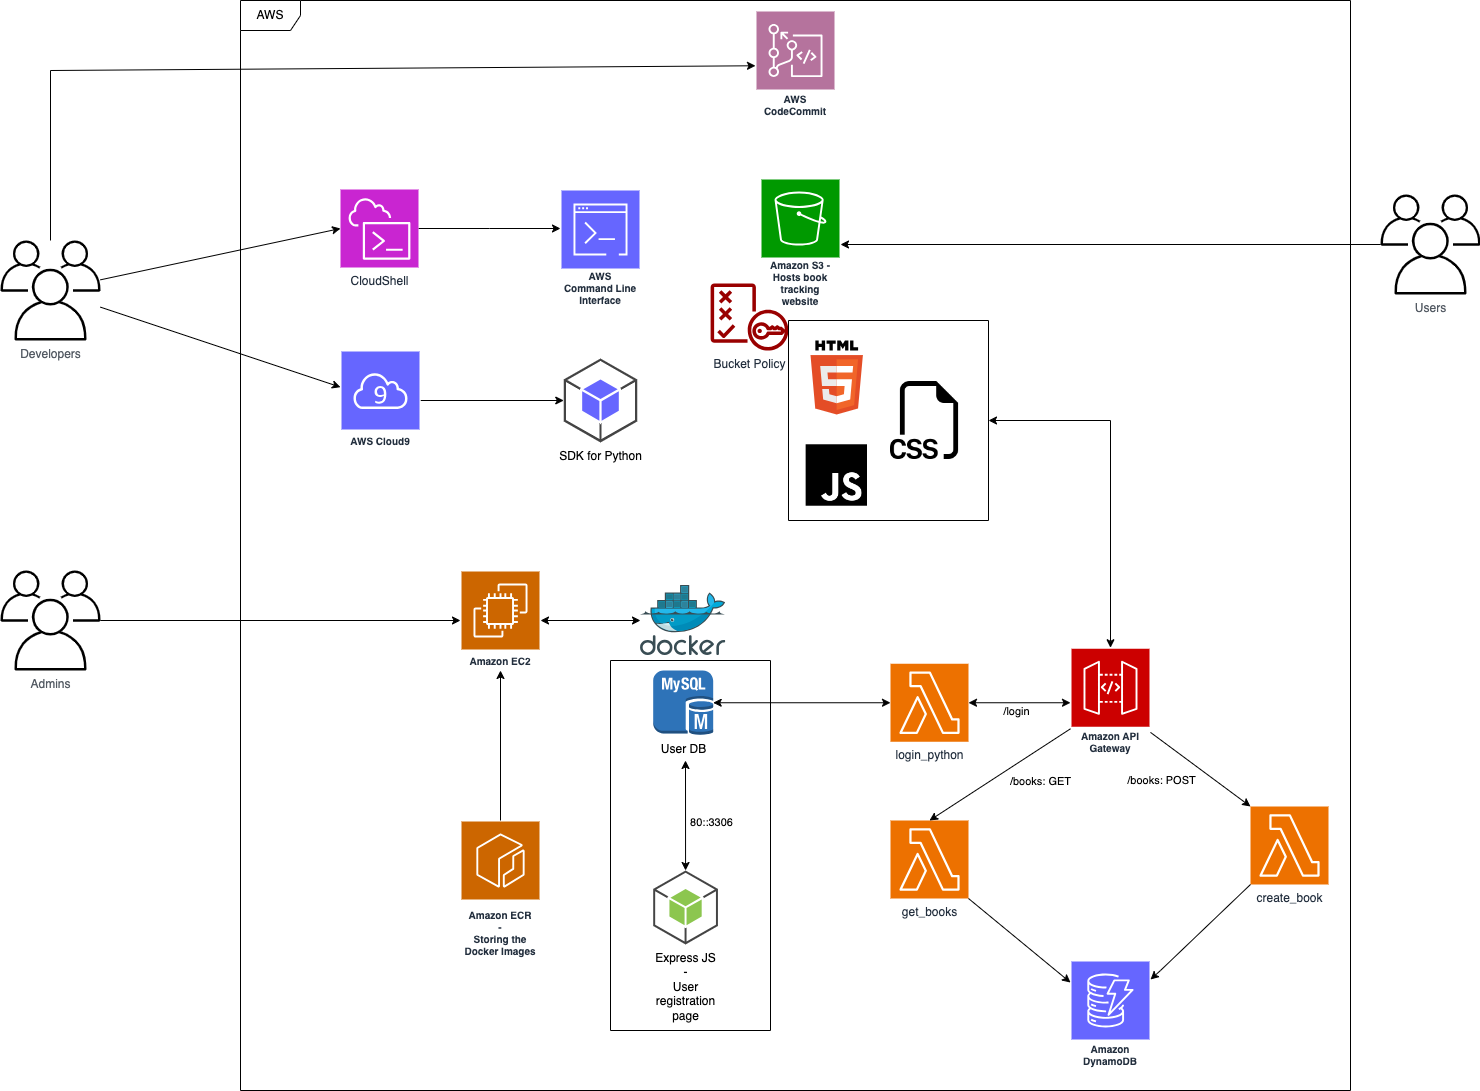
\includegraphics[scale=0.23]{aws.drawio.png}
  \caption{The architecture of the application.}
  \label{fig:TexnicCenter}
\end{figure}

\section{Docker}

Docker is a set of platform as a service (PaaS) products that use OS-level virtualization to deliver software in packages called containers. Containers are isolated from one another and bundle their own software, libraries and configuration files; they can communicate with each other through well-defined channels. All containers are run by a single operating system kernel and are thus more lightweight than virtual machines. Containers are created from images that specify their precise contents. Images are often created by combining and modifying standard images downloaded from public repositories. \cite{docker}
I used this for the admin page creation and for storing the user data in a MySQL database. I created two containers, one for the admin page and one for the database. The admin page is written in Express JS and the database is MySQL.

\subsection{MySQL - User database}

MySQL is an open-source relational database management system (RDBMS). Its name is a combination of "My", the name of co-founder Michael Widenius's daughter, and "SQL", the abbreviation for Structured Query Language. A relational database organizes data into one or more data tables in which data types may be related to each other; these relations help structure the data. SQL is a language programmers use to create, modify and extract data from the relational database, as well as control user access to the database.
I have set up this database using Docker and I have created a table for the users. The table has the following columns: username, password. To create the container I first created the image, which is created from the Dockerfile. The Dockerfile I composed contains the fondamentals like it used mysql 8.2.0 and it exposes its port to 3306.
After the creation I used the following command to update the database.
\begin{lstlisting}[language=Python,basicstyle=\ttfamily\small,]
  docker run --name mysql_1 -p 3306:3306 
    -> -e MYSQL_ROOT_PASSWORD=pwd -d mysql_server
  docker exec -i mysql_1 mysql -u root -ppwd < db.sql
\end{lstlisting}
After I have successfuly created the container I tagged it and pushed it to the AWS ECR(Elastic Container Registry).

\begin{lstlisting}[language=Python,basicstyle=\ttfamily\small,]
  docker tag mysql_server 
    -> 554751627586.dkr.ecr.eu-north-1.amazonaws.com/mysql_1:latest
  docker push 554751627586.dkr.ecr.eu-north-1.amazonaws.com/mysql_1:latest
\end{lstlisting}

\subsection{Express JS - Admin page}

The admin front end page was developed using Express JS. Express is a minimal and flexible Node.js web application framework that provides a robust set of features for web and mobile applications.
On the webpagee the admins can register new users and also delete them. The users and their passwords are stored in the MySQL database. I also applied Bootsraps to the page to make it more user friendly and responsive.
After I have finished the development I have created the image and pushed it to the AWS ECR(Elastic Container Registry) also.
\begin{lstlisting}[language=Python,basicstyle=\ttfamily\small,]
  docker inspect network bridge
  docker build --tag node_app .   
  docker run -d --name node_app_1 -p 3000:3000 
    -> -e APP_DB_HOST=172.17.0.2 node_app
\end{lstlisting}

I exposed the 3000 TCP port to the 3000 port of the host machine. I also set the APP\_DB\_HOST environment variable to the IP address of the MySQL container.
This way the Express JS application can connect to the MySQL database.

\section{Amazon EC2 - Elastic Compute Cloud}
Aftr I have pushed my conatainers to the AWS ECR I have created an EC2 instance. I have used the Amazon Linux 2 AMI (HVM), SSD Volume Type. I have also added a 30GB storage to the instance. I have also added that the the instance can be accessed from anywhere. So I added a Security Group with the following rules:
\begin{itemize}
  \item SSH - TCP - 22 - Anywhere
  \item HTTP - TCP - 80 - Anywhere
  \item HTTPS - TCP - 443 - Anywhere
  \item MYSQL/Aurora - TCP - 3306 - Anywhere
\end{itemize}

After the creation of the instance I have connected to it using SSH. I have also installed Docker and Docker Compose on the instance. After that I have pulled the images from the AWS ECR and started the containers. I also had to authorize the Docker to pull images from the AWS ECR. I have done this by running the following command:

\begin{figure}[h]
  \centering
  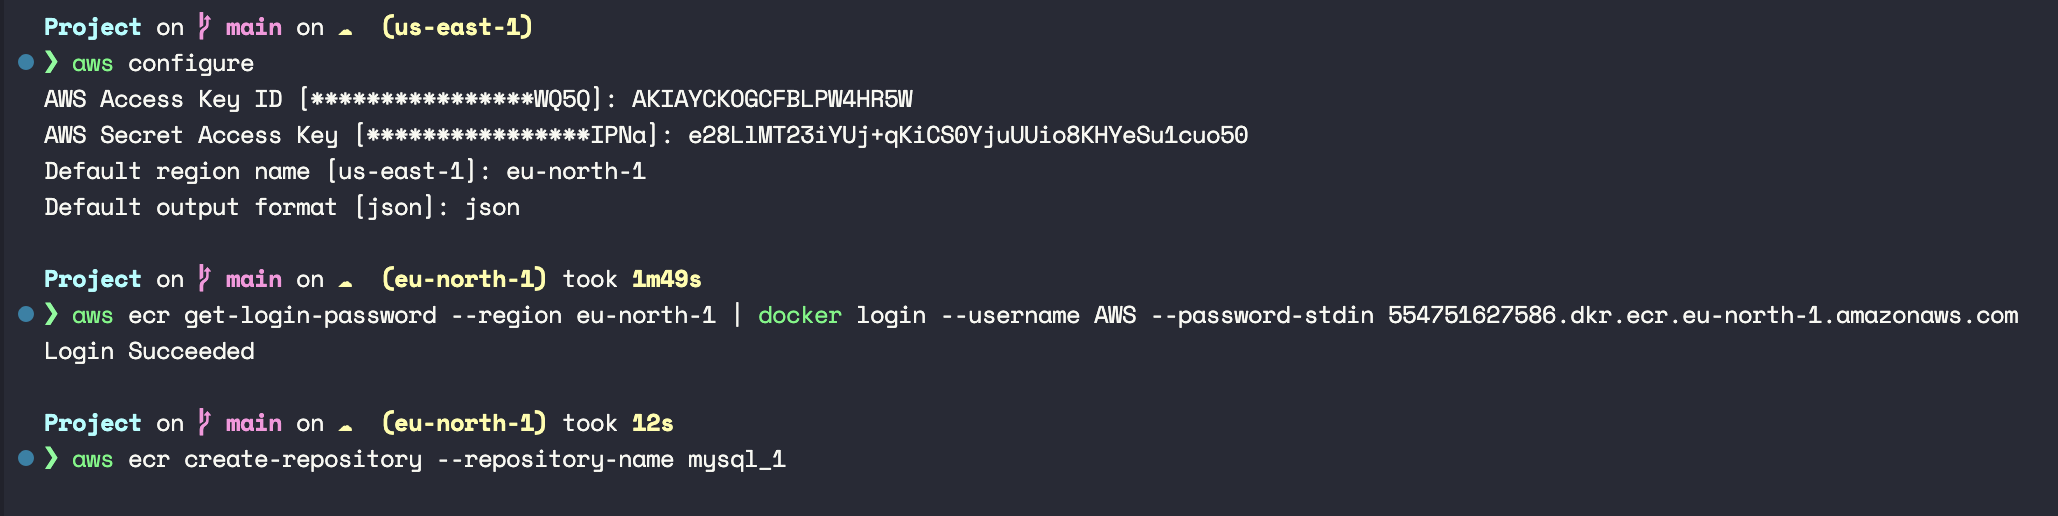
\includegraphics[scale=0.45]{aws_configure_ec2.png}
  \caption{AWS EC2 configuration.}
  \label{fig:TexnicCenter}
\end{figure}

\begin{lstlisting}[language=Python,basicstyle=\ttfamily\small,]
  aws ecr get-login-password --region eu-north-1 
  docker login --username AWS --password-stdin 
    -> 554751627586.dkr.ecr.eu-north-1.amazonaws.com
  docker pull 554751627586.dkr.ecr.eu-north-1.amazonaws.com/node-app
\end{lstlisting}



After this I started the front-end page of the Book Tracking app.

\section{Amazon S3 - Simple Storage Service}

The front-end page for the Book Tracking app is hosted on the Amazon S3. I have created a bucket for the page and I have uploaded the files to the bucket. I have also set the bucket to be public so anyone can access it. I have also set the bucket to be a static website hosting. I have also set the index.html as the index document. This way the page will be loaded when the user enters the URL of the bucket.
The page was creste with the help of HTML, CSS and JavaScript. I have also used Bootstrap to make the page more user friendly and responsive. First the user has to log in to the page.
This data is stored in the MySQL database. After the successful login the user can see the books he/she has added to the list.
The books are stored in the Amazon DynamoDB database. The user can also log out from the page.
When the login happens or the Amazon DynamoDB retrieval the page sends a request to the Amazon API Gateway. This is a REST API which is connected to the AWS Lambda function. This function is written in Python and it is responsible for the communication between the front-end page and the Amazon DynamoDB database. The function is also responsible for the authentication of the users.
In the next section I will explain these.

\section{Amazon API Gateway}

The Amazon API Gateway is used to host the different ReST APIs. There I have created the following APIs:
\begin{itemize}
  \item GET: books
  \item POST: create\_book
  \item GET: login
\end{itemize}

To create these APIs I have used the AWS Lambda functions. I have also set the API Gateway to be public so anyone can access it. I have also set the CORS to be enabled. This way the front-end page can access the APIs. I have also set the API Gateway to be a proxy. This way the API Gateway will forward the requests to the AWS Lambda functions. I have also set the API Gateway to be a REST API. This way the API Gateway will be able to handle the different HTTP methods.

\begin{figure}[!ht]
  \centering
  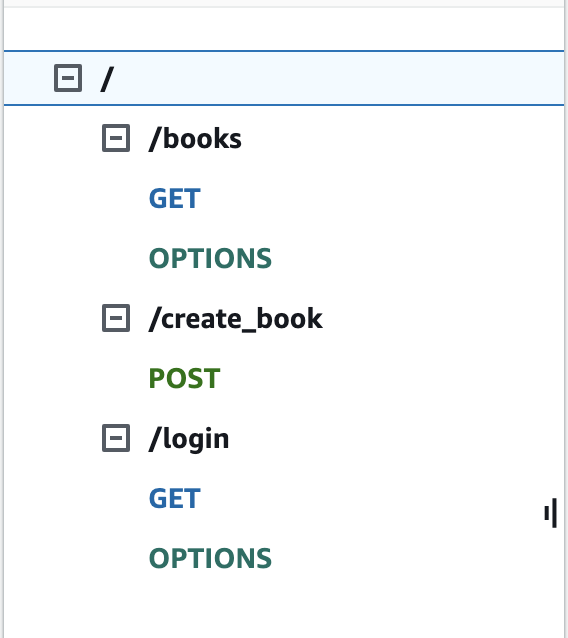
\includegraphics[scale=0.5]{api.png}
  \caption{The APIs for the application.}
  \label{fig:TexnicCenter}
\end{figure}

\section{AWS Lambda}

For the APIs i have created the following AWS Lambda functions:
\begin{itemize}
  \item get\_books - is used for the GET: books API. It is responsible for retrieving the books from the Amazon DynamoDB database.
  \item post\_book - is ued for the POST: create\_book API. It is responsible for creating a new book in the Amazon DynamoDB database.
  \item login\_python - is used for the GET: login API. It is responsible for the authentication of the users.
\end{itemize}

These lambda functions were created using Python. For the login python I had to create a Lambda Layer. The layer was needed to add mysql.connector to the Lambda function. This way the function can connect to the MySQL database. I have also set the timeout for the functions to be 30 seconds. This way the functions will not time out when they are retrieving the data from the database.

\begin{figure}[!ht]
  \centering
  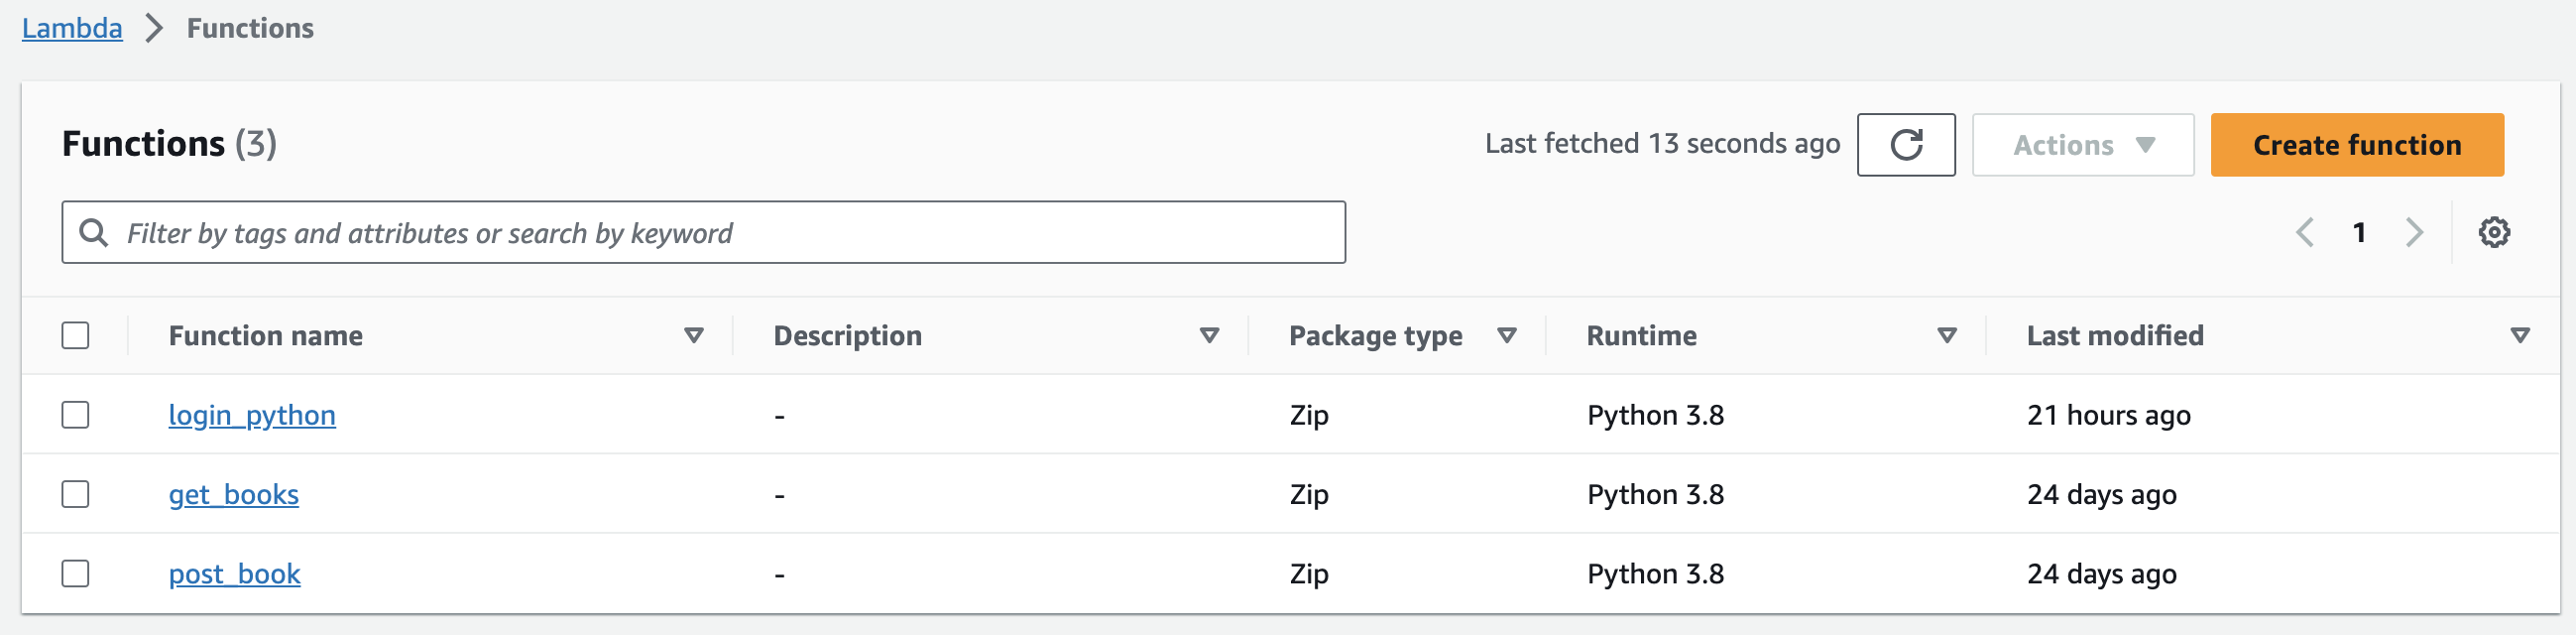
\includegraphics[scale=0.4]{lambda_functions.png}
  \caption{The lambda functions for the APIs.}
  \label{fig:TexnicCenter}
\end{figure}


\chapter{Presentation of finished work}

In this section I will present and showcase my finished appliction. I will include screenshots to have a better representation and understanding for the reader.


\begin{figure}[!ht]
  \centering
  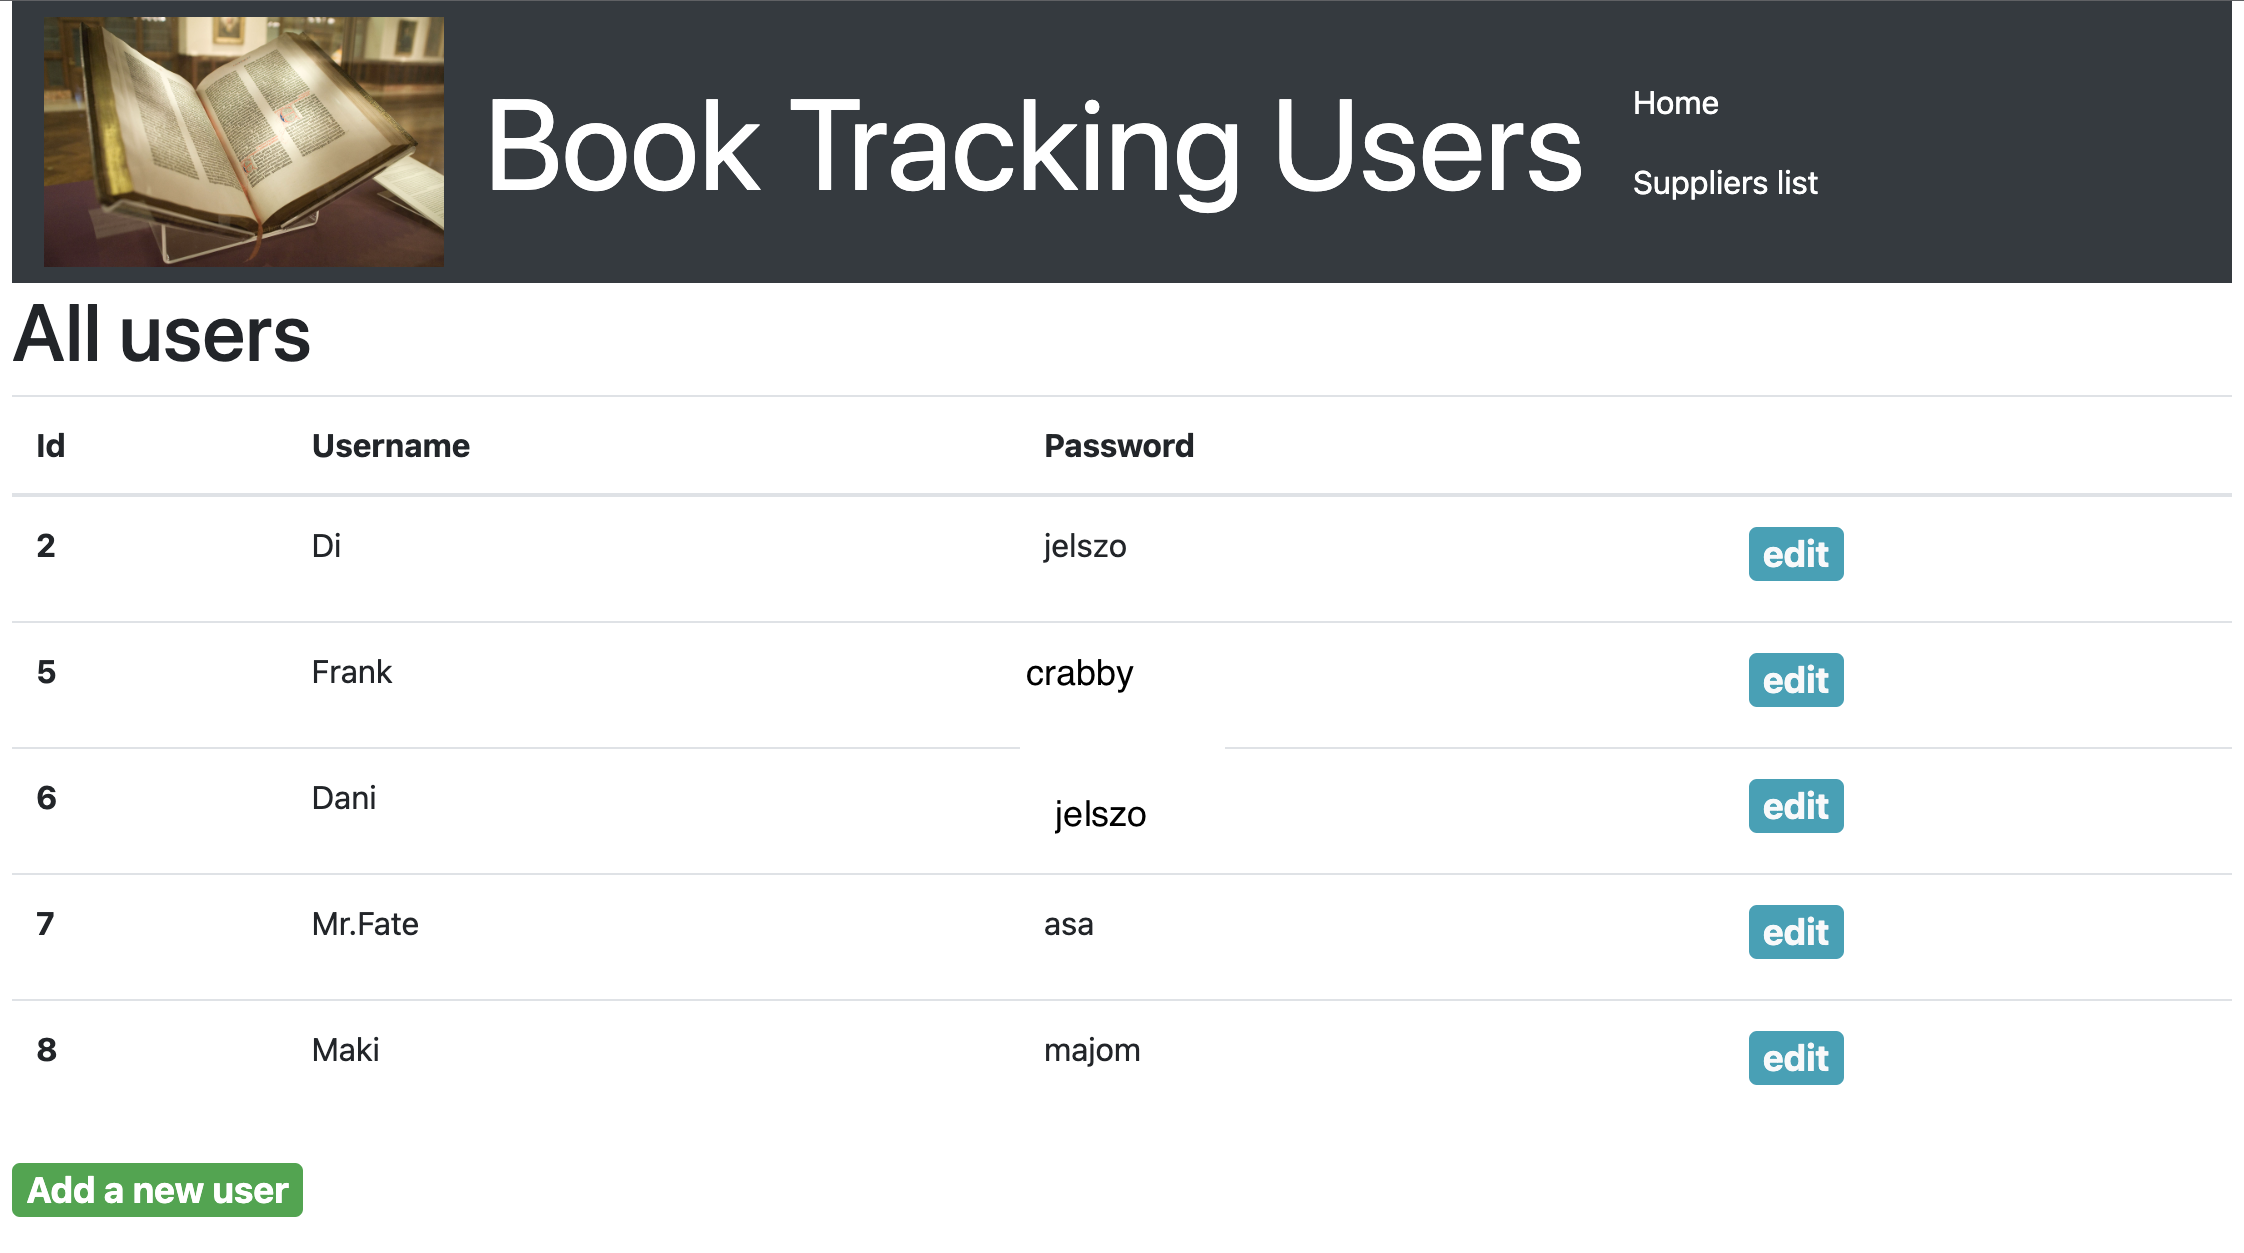
\includegraphics[scale=0.3]{admin_list.png}
  \caption{The main screen of the admin page.}
  \label{fig:TexnicCenter}
\end{figure}

\begin{figure}[!ht]
  \centering
  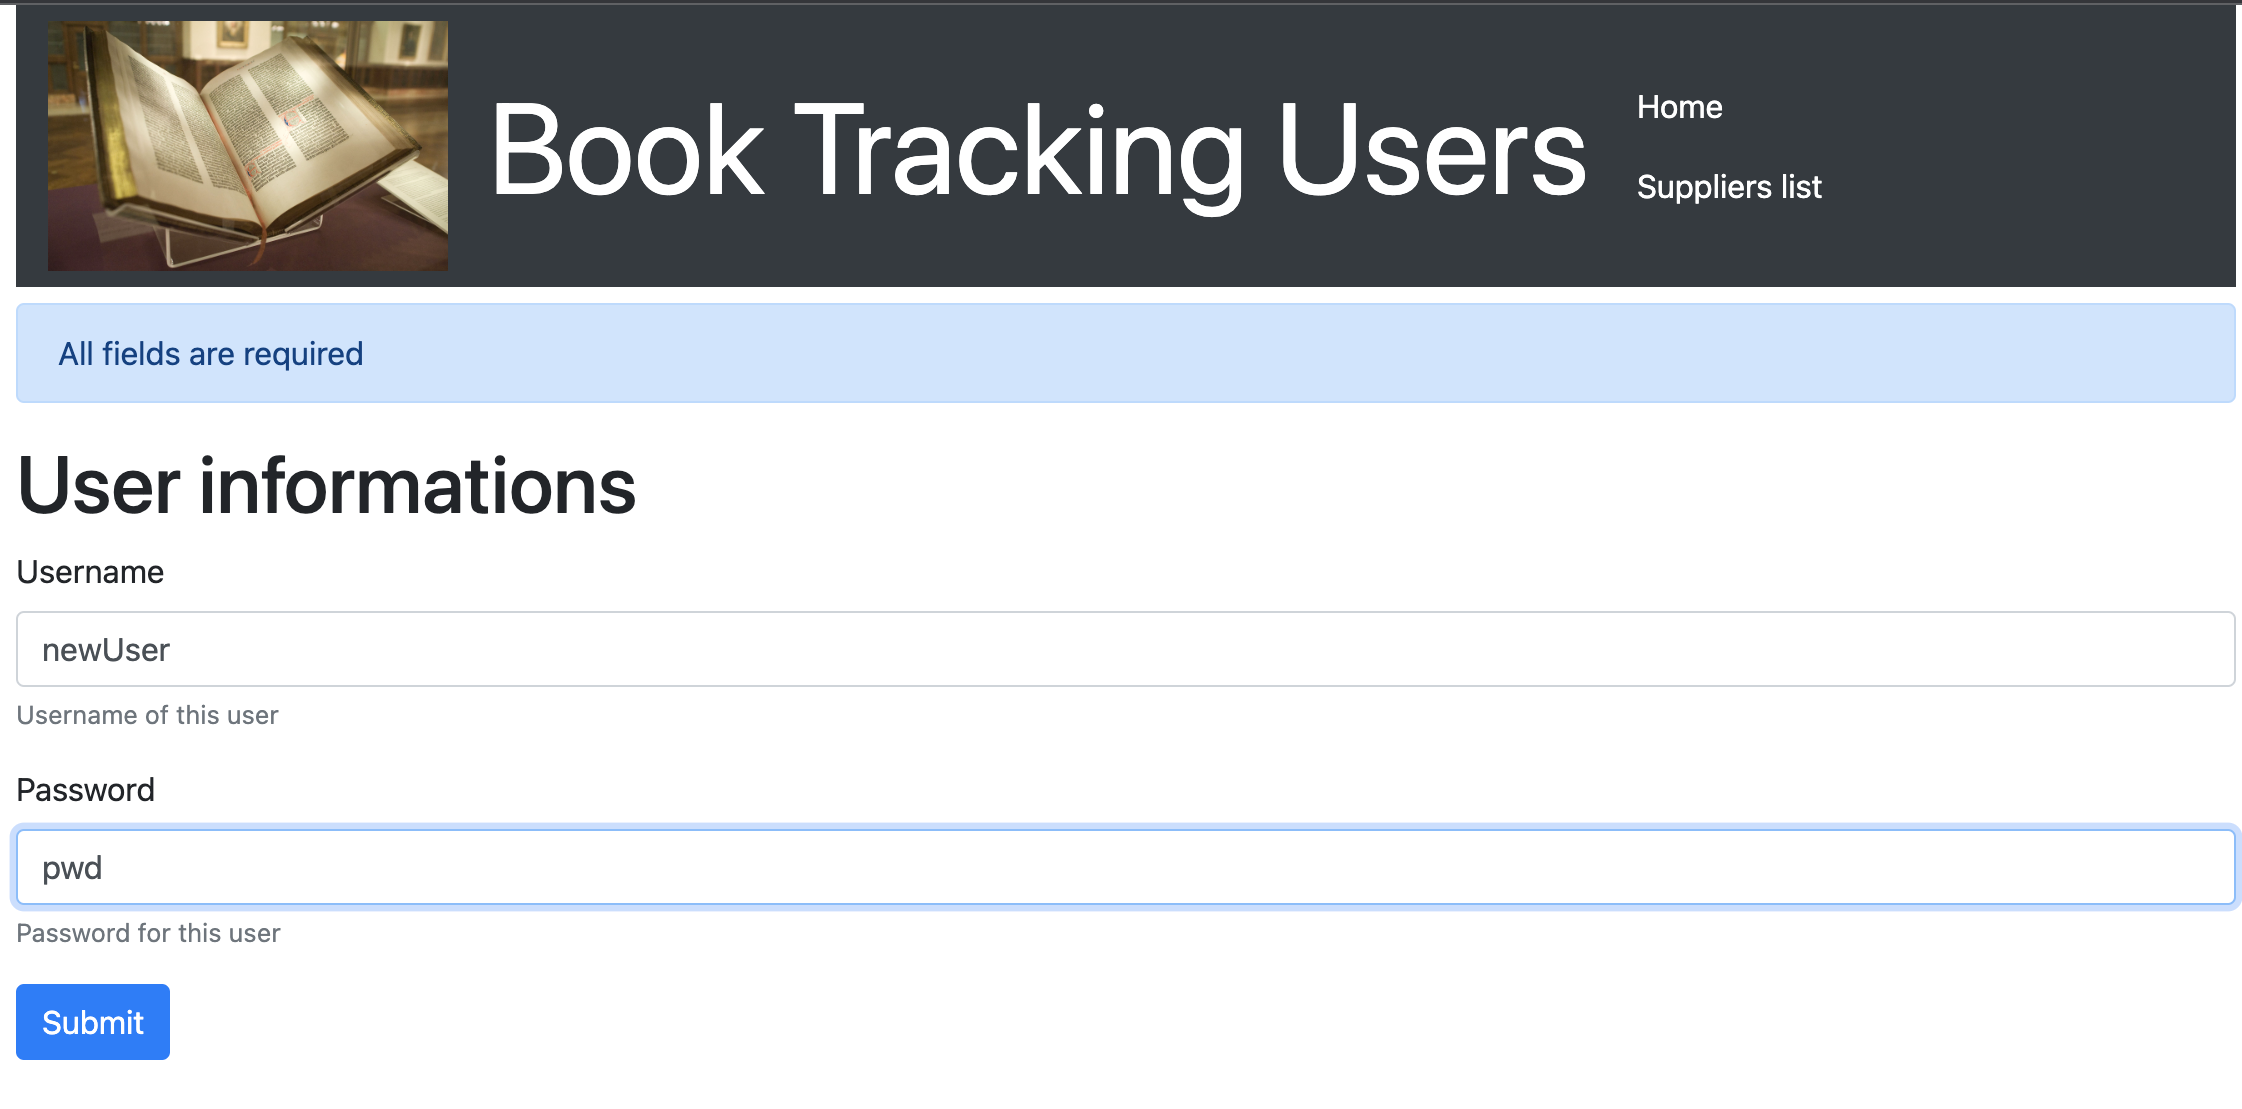
\includegraphics[scale=0.3]{admin_create.png}
  \caption{Creating a new user.}
  \label{fig:TexnicCenter}
\end{figure}

\begin{figure}[!ht]
  \centering
  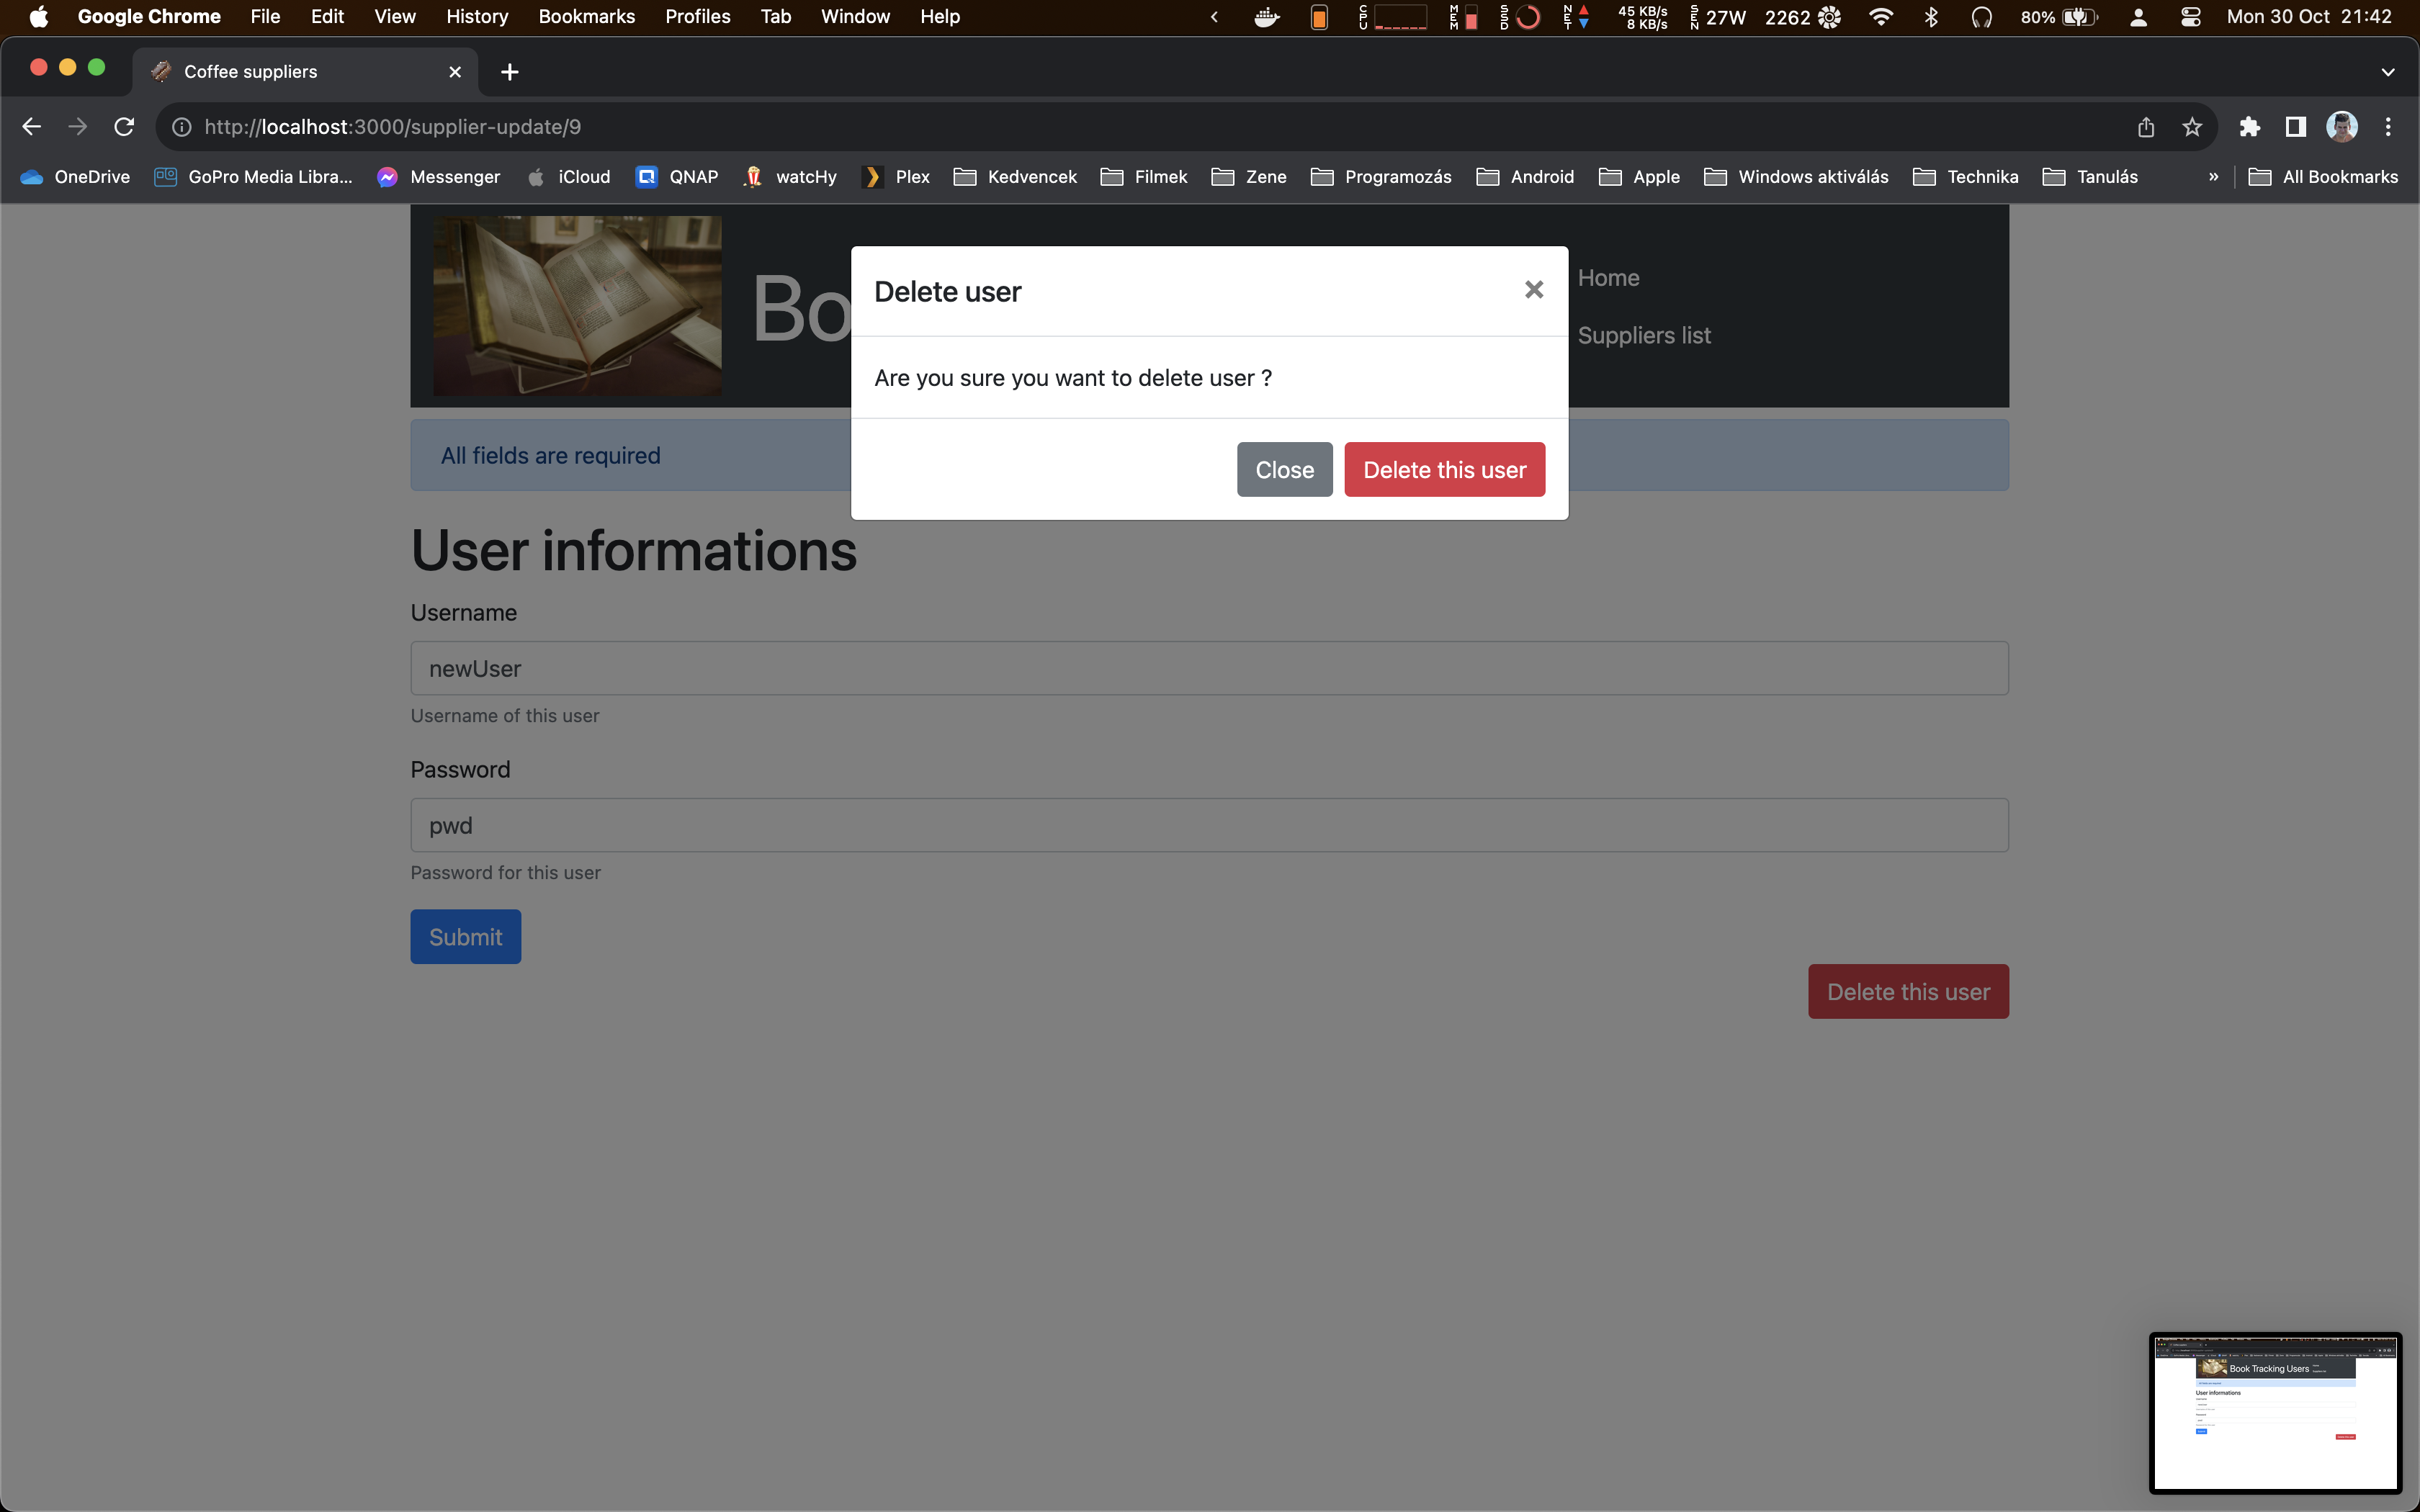
\includegraphics[scale=0.3]{admin_delete.png}
  \caption{Deleting a user.}
  \label{fig:TexnicCenter}
\end{figure}


\begin{figure}[!ht]
  \centering
  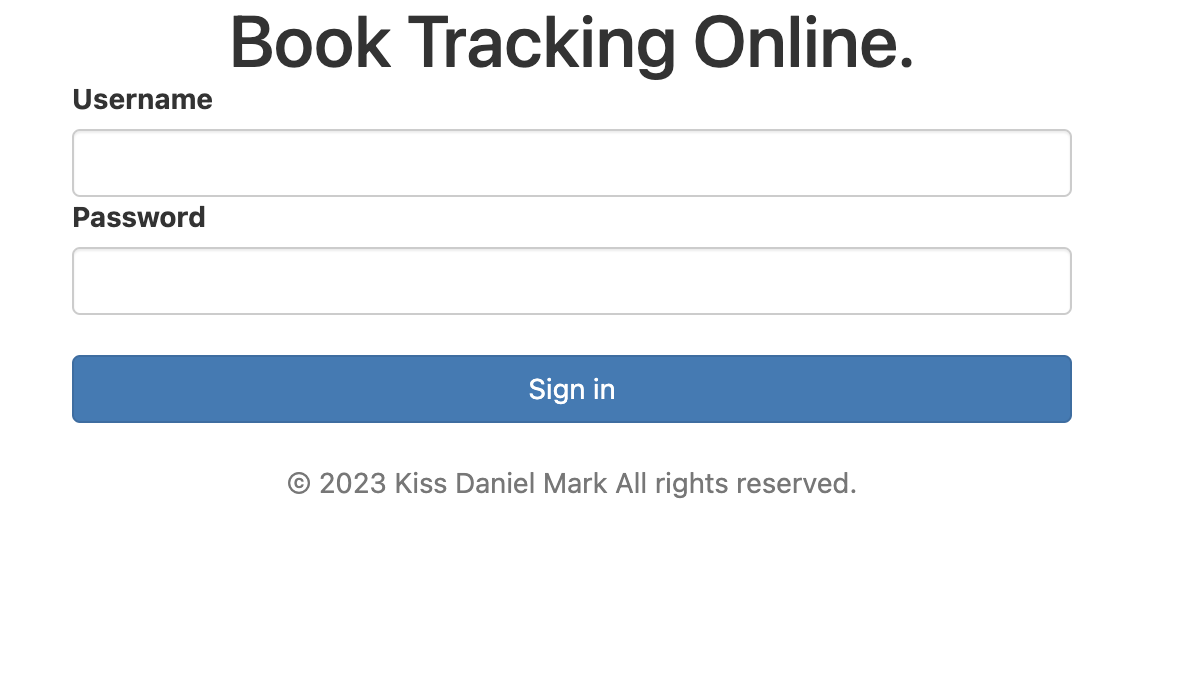
\includegraphics[scale=0.3]{frontend-login.png}
  \caption{The login page of the application.}
  \label{fig:TexnicCenter}
\end{figure}

\begin{figure}[!ht]
  \centering
  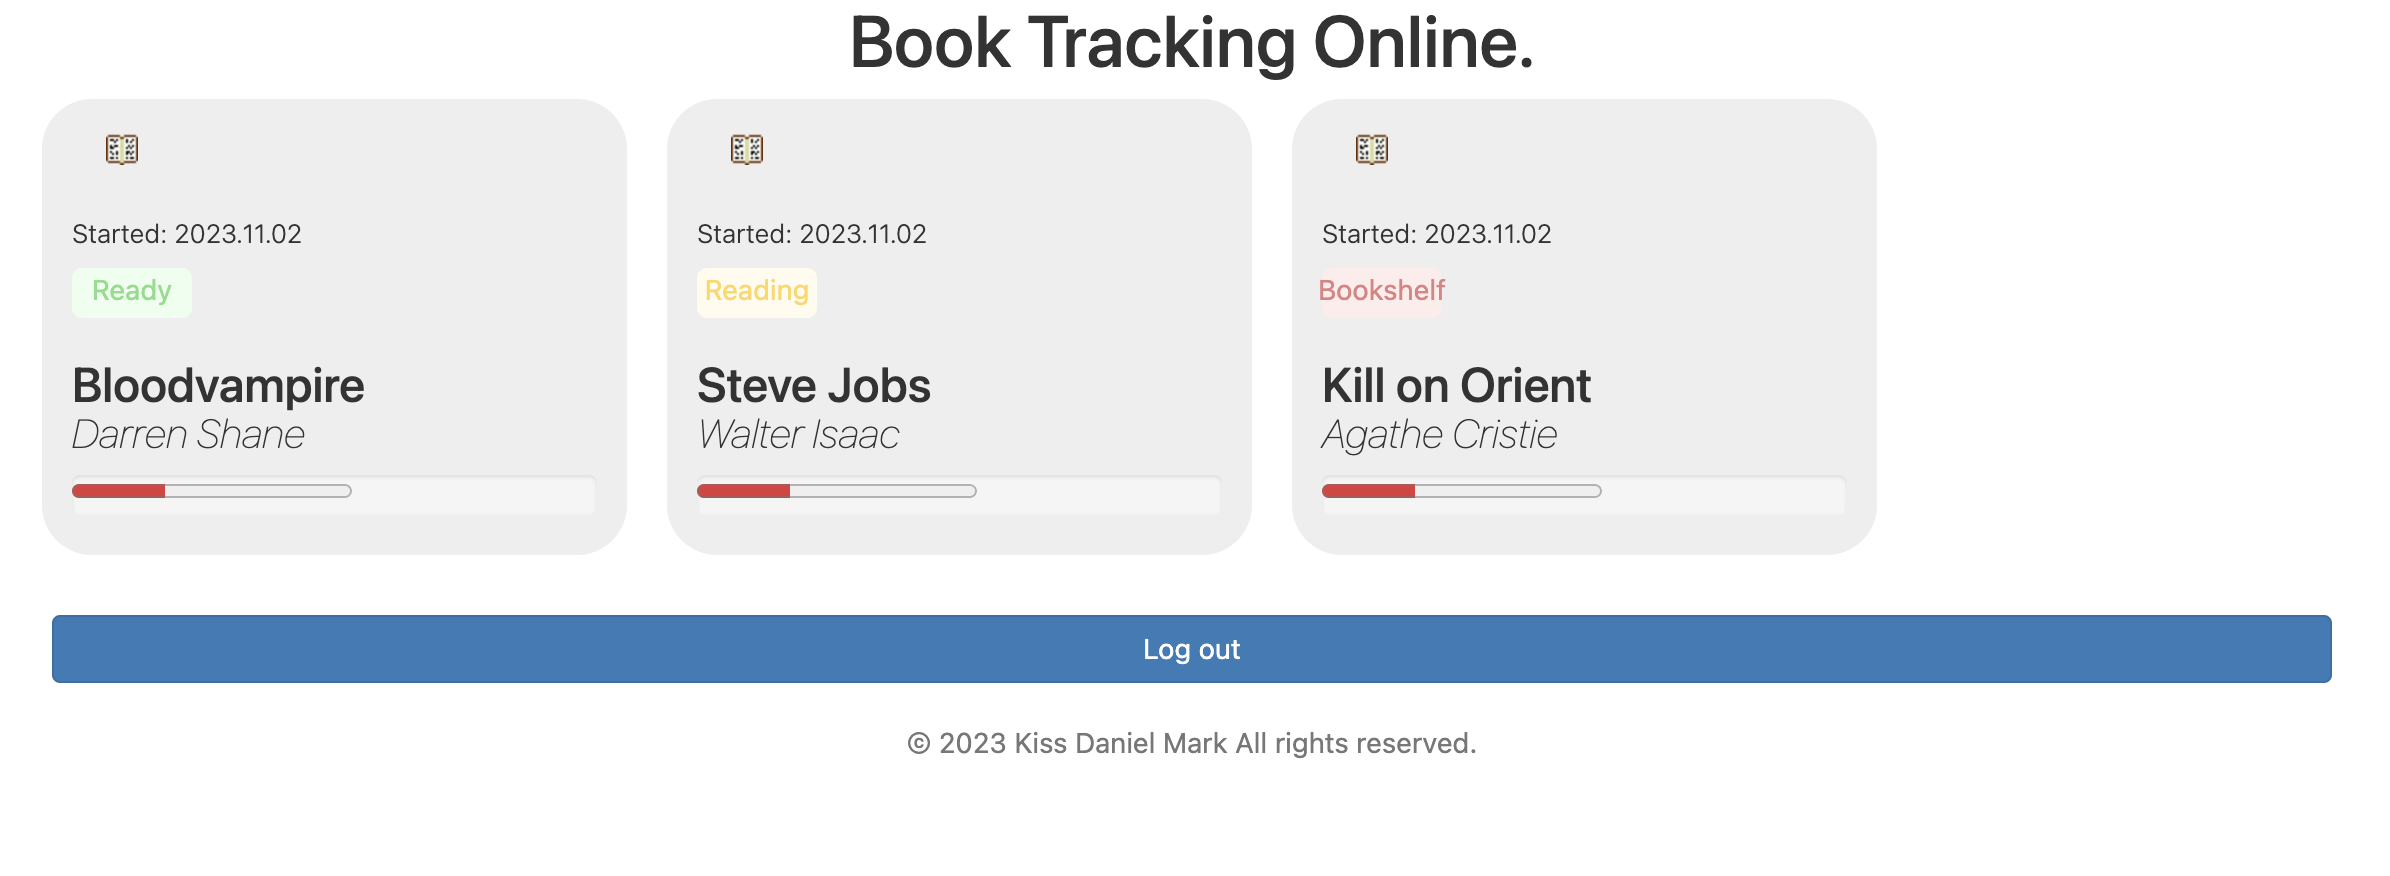
\includegraphics[scale=0.3]{frontend-main.png}
  \caption{The main screen of the application.}
  \label{fig:TexnicCenter}
\end{figure}

\begin{thebibliography}{9}
  \bibitem{techtagaws}
  TechTarget - Amazon Web Services: https://www.techtarget.com/searchaws/definition/Amazon-Web-Services

  \bibitem{awsacademy}
  Amazaon Web Services Academy: https://aws.amazon.com/training/awsacademy/

  \bibitem{awsec2}
  Amazon EC2: https://aws.amazon.com/pm/ec2/

  \bibitem{awss3}
  Amazon S3: https://aws.amazon.com/s3/

  \bibitem{awsrds}
  Amazon RDS: https://aws.amazon.com/rds/

  \bibitem{awsddb}
  Amazon DynamoDB: https://aws.amazon.com/dynamodb/

  \bibitem{awslambda}
  Amazon Lambda: https://aws.amazon.com/lambda/

  \bibitem{awscodecommit}
  Amazon CodeCommit: https://aws.amazon.com/codecommit/

  \bibitem{docker}
  Docker: https://www.docker.com


\end{thebibliography}

\end{document}


%%drawio ábra
%%prcie calculator
%%improvements
